\documentclass[10pt]{article}

\usepackage{amsmath}

\newcommand{\myvec}[1]{\ensuremath{\begin{pmatrix}#1\end{pmatrix}}}

\newcommand{\mydet}[1]{\ensuremath{\begin{vmatrix}#1\end{vmatrix}}}

\newcommand{\solution}{\noindent \textbf{Solution: }}

\providecommand{\brak}[1]{\ensuremath{\left(#1\right)}}

\providecommand{\norm}[1]{\left\lVert#1\right\rVert}
\usepackage{graphicx}
\usepackage{float}

\let\vec\mathbf
\title{Coordinate Geometry}
\author{harshita (paidisettyharshita@sriprakashschools.com)}

\begin{document}
\maketitle
\section*{Class 10$^{th}$ Maths - Chapter 7}
This is Problem-7 from Exercise 7.4
\begin{enumerate}
\item Find the coordinates of a point A, where AB is the diameter of a circle whose centre is (2, -3) and B is (1, 4).\\

\solution:
\begin{align}
  \vec{C} &= \frac{m\vec{B}+n\vec{A}}{m+n}\\
\vec{C}m+\vec{C}n&=m\vec{B}+n\vec{A}\\
\frac{\vec{C}m+\vec{C}n-\vec{m}B}{n}&=\vec{A}\\
\end{align}

\begin{align}
\vec{C} &= \myvec{2\\-3}\\
\vec{B} &= \myvec{1\\4} \\
\end{align}
By taking m=1 and n=1
\begin{align}
so,\\
\vec{A}&=\frac{\myvec{2\\-3}+\myvec{2\\-3}-\myvec{1\\4}}{1}\\
\vec{A}&=\myvec{3\\-10}
\end{align}


\end{enumerate}
\begin{figure}[H]
			\centering
			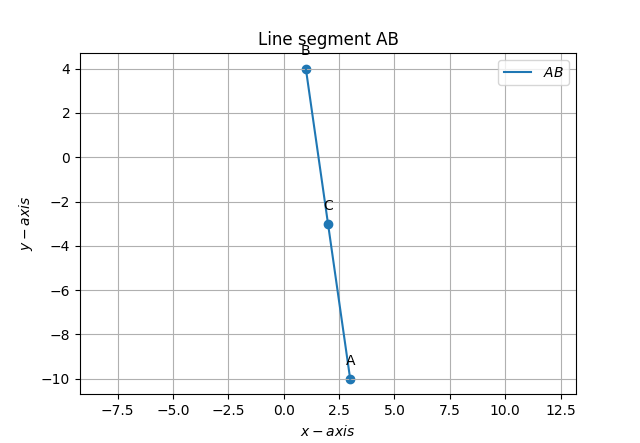
\includegraphics[width=\columnwidth]{figs/Figure_1.png}
			\caption{Line segment AB}
			\label{fig:5}
		\end{figure}
\end{document}
